\section{Design Specification}
    In this section, overall design of the project is discussed, presenting arguments for various choices made and the outcomes of such choices. Existing and possible dependencies, constraints or limitations are mentioned here.
    
    The \nameref{techstack} subsection presents various technologies chosen to develop the software and fulfil the requirements specified in previous chapters.
    
    The \nameref{assumptionsdependencies} subsection discusses how current design impacts the software's dependencies and installation process.
    
    The \nameref{designconstraints} subsection gives an overview of limitations with regards to software use cases and possible challenges to the user. 
    
    \subsection{Technology Stack} \label{techstack}
        Technological choices are presented and explained here in detail. Alternatives are also discussed and argued for and against. This section covers the discussions of Programming Languages, Dependency and Package Managers, and Programming Libraries.
        
        \subsubsection{Programming Language}
            Programming language Python version 3.7. There is a reason why Python is the de facto language for all purposes Machine Learning, Deep Learning, Data Science and Analysis, and this is because of the vast amount of libraries that enable the developer to easily incorporate the functionality in any project. Nonetheless, the core calculations of those libraries are done in C/C++ language and Python is used as a wrapper for easy access and compatibility, which makes memory intensive computations all the more efficient. 
            
            Even though C/C++ offers much more flexibility in terms of memory management and performance optimisation, the core data science and machine learning libraries and frameworks, for historical reasons, are mostly saturated in Python language, while C/C++ is left as more of a pure hardware and game development language. Additionally, Python requires less code and its' syntax is less strict, which is probably why it is a popular language among research communities, allowing for faster prototyping of new algorithms and ideas.
            
            Older version of Python2.7 is still a popular alternative. Currently, most of the frameworks and libraries are still supporting this version of Python, as well as there are older frameworks that have not yet updated to be compatible with version 3.7 and are only available on 2.7. But with Python2.7 being quite old in technology terms and some framework developers announcing that in a couple of years they will not be supporting Python2.7 anymore makes this a less attractive option. There are also syntactical differences between versions, with Python3.7 offering a more cleaner and concise coding options. Overall, Python2.7 is supported today only because of backward compatibility reasons and not because it is being developed or updated independently by the language creators.
        
        \subsubsection{Dependency and Package Managers}
            Anaconda was used as a package and dependency manager for Python, allowing easy and quick addition of various external libraries (Tweepy, TensorFlow and various sub dependencies). Moreover, PyCharm was used to fulfil the role of Integrated Development Environment for Python, mostly because of it having a lot more features than the free counterparts, as students can get Ultimate license free of charge for a year. Alternatively, Python has PIP which is also a package manager, albeit more lightweight in that it is purely a command line interface. Anaconda comes with a graphical interface and a prepackaged bundle of most common libraries, which are not included if PIP was chosen as default package manager.
            
        \subsubsection{Twitter Data Access Library}
            Tweepy was chosen to be used as Twitter API access library, because, first of all, is one of the not many libraries that are still maintained and updated today, constantly providing more and more flexibility with gathering of Twitter Data, and secondly, because of documentation providing lots of examples how to quickly set up and get up to speed. An alternative could have been to create a custom \gls{api} to access twitter posts. This would have led to more flexibility from development point of view, but increased time spend developing it is not worth it as existing solution proves sufficient for the task at hand.
            
        \subsubsection{Deep Neural Network Development Library Framework}
            The most popular library that delivers upon the objectives of the project is TensorFlow, and as such it is used in this project. It's popularity speaks volumes as there is a vast amount of guides easily accessible and extendable into solving complex problems (such as Recognizing Textual Entailment, for example). Also, the documentation is full with up to date details and examples clearly explaining differences between previous and future (yet to be released) versions. Another popular library is PyTorch, it also features a lot of functions that can perform the same tasks as TensorFlow. Difference being that PyTorch is a newer framework, naturally meaning smaller community and lesser flexibility (at least until it has fully caught up to existing TensorFlow framework), but it is offering new ways of doing things (in some functions) which may prove useful in some cases. The verdict is that currently, TensorFlow offers higher control of parameter tuning for the purpose of training and developing \gls{lstm} networks.
        
    \subsection{Assumptions and Dependencies} \label{assumptionsdependencies}
        
        \subsubsection{Software Installation}
            Open source, no installation, manual dependency management.
    
    \subsection{Design and Implementation Constraints} \label{designconstraints}
        
        \subsubsection{User Interface}
            everything is through command line interface.
        
        \subsubsection{Use of Software}
            not suited for marketing currently, but can be used by people with technological background.
    

    
    
% The chapter reports the contribution of your work.  For example, it could contain the following sub-sections to summarise the contribution of the project: Theoretical Development, Analysis and Design, Implementation and Experimental Work, Results, Observation and Discussion.

% \subsection{Maths}
% \begin{equation}\label{eq:BS}
% \frac{\D S_t}{S_t} = r \D t + \sigma \D W_t,
% \qquad S_0>0,
% \end{equation}

% The equation $\sigma = m a$ follows easily~\citep{phdthesis}.

% \subsection{Glossary and acronyms}

% \Glspl{Linux} and other Unix operating systems are better then Windows because they support \gls{lvm} out of the box~\citep{Joh11}\insertref{reference missing}. 

% \subsection{Figures}
% Here is an example of how to insert a picture:

% \begin{figure}[!ht]
% \centering
% \subfigure{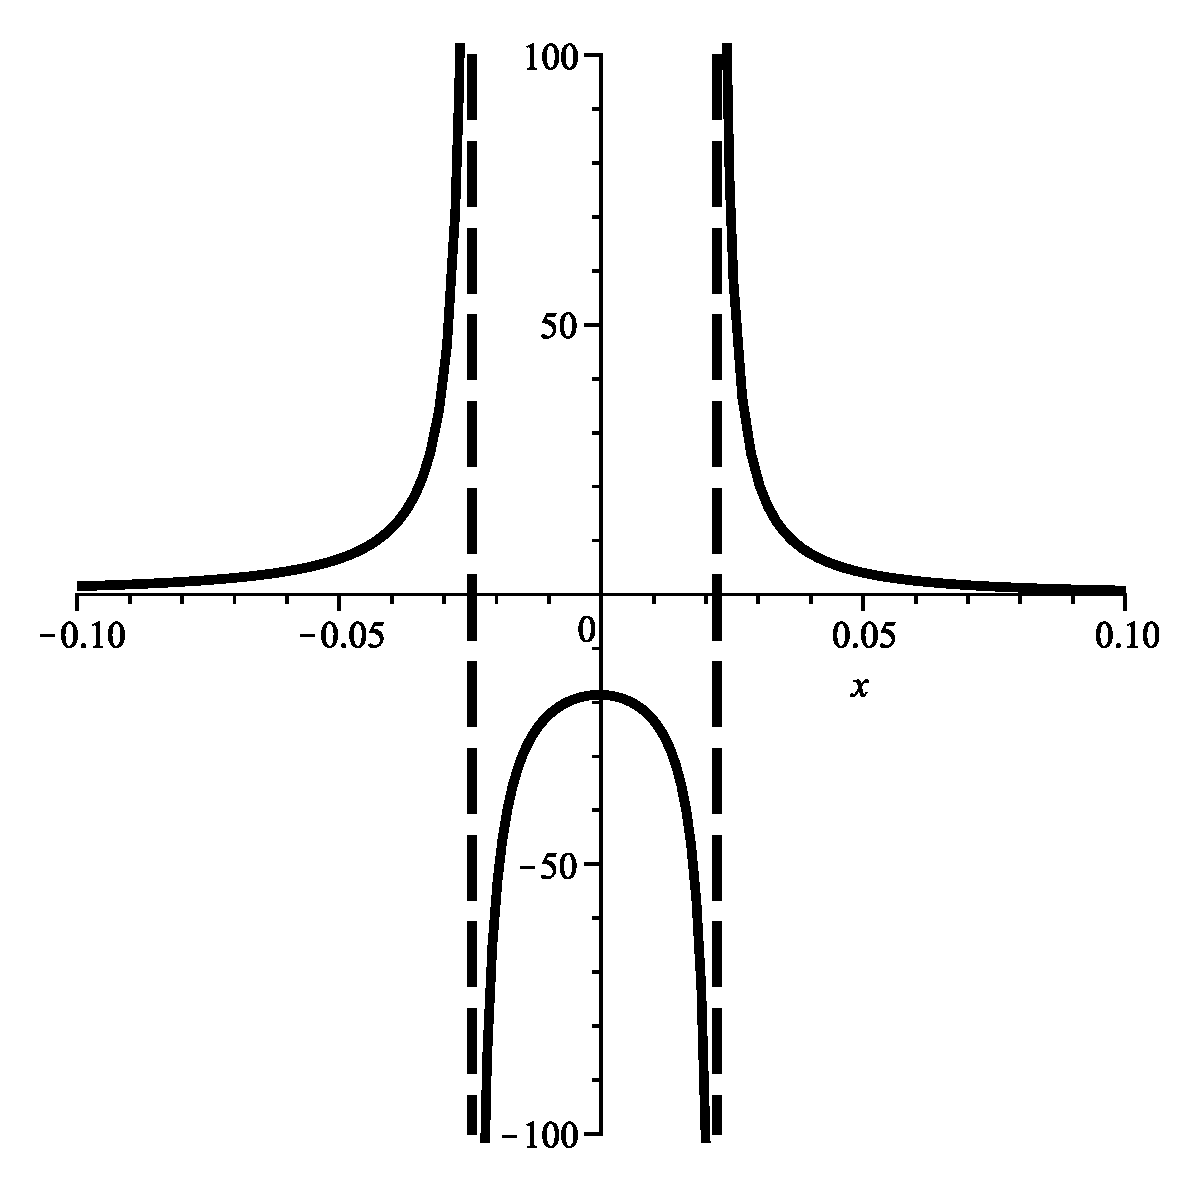
\includegraphics[scale=0.2]{figures/Picture.eps}}
% \caption{This is the caption for the figure.}
% \label{fig:Pict}
% \end{figure}


% \begin{figure}[!ht]
% \centering
% \missingfigure{If you know there will be a figure, but you still need to create it.}
% \caption{This is the caption for the figure which is not even present.}
% \label{fig:PictMis}
% \end{figure}

% \todo{This is a small Todo, please take care!}

% or two side-by-side pictures:

% \begin{figure}[!ht]
% \centering
% \subfigure{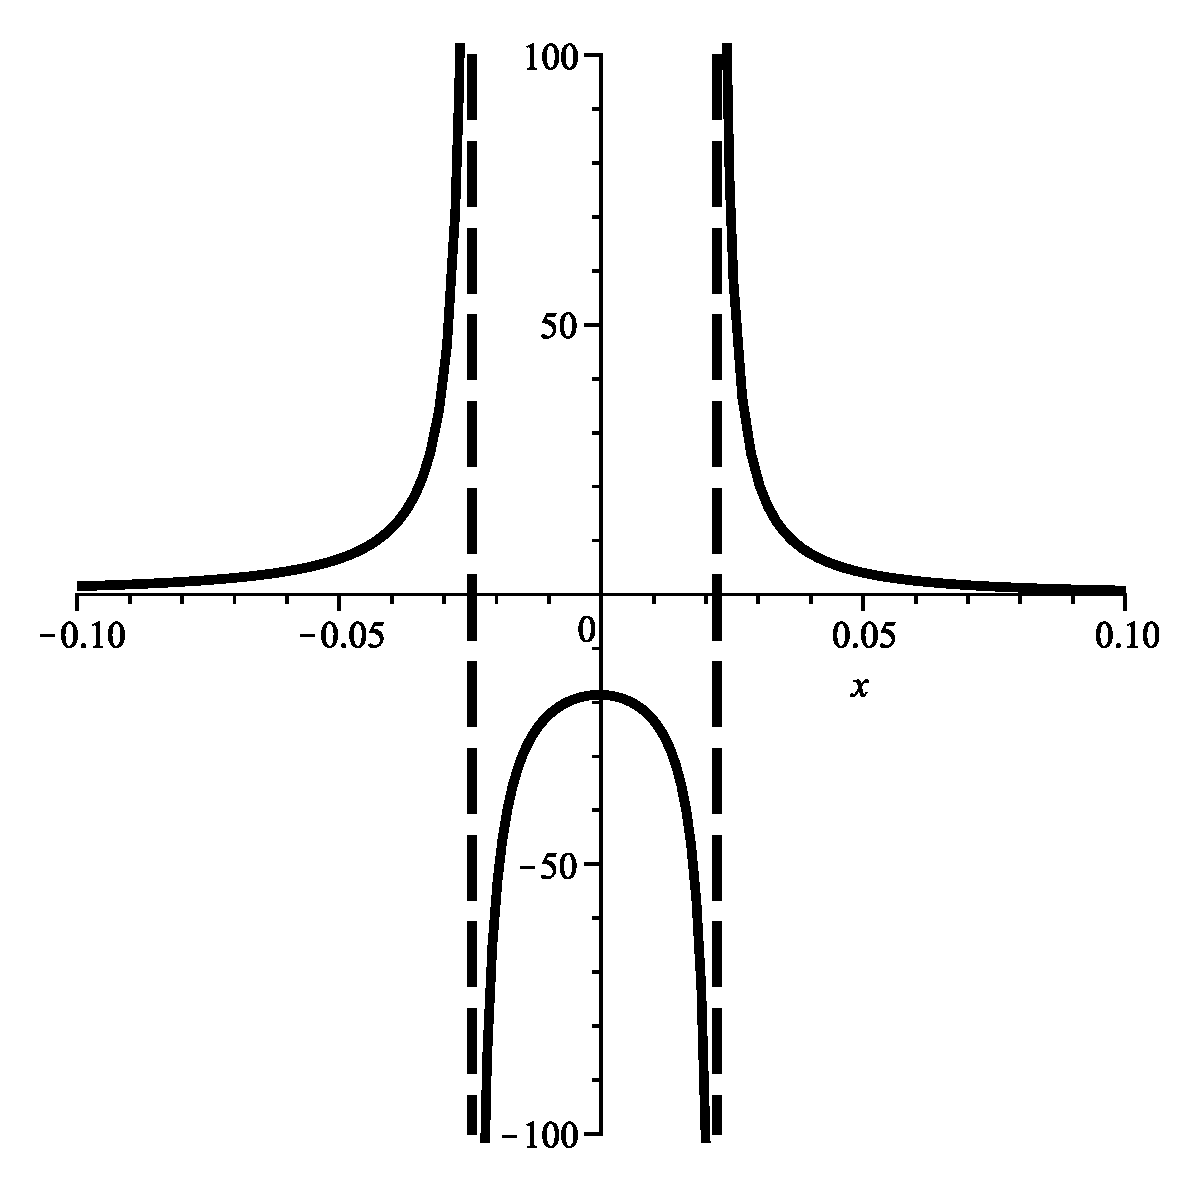
\includegraphics[scale=0.3]{figures/Picture.eps}}
% \hspace{15pt}
% \subfigure{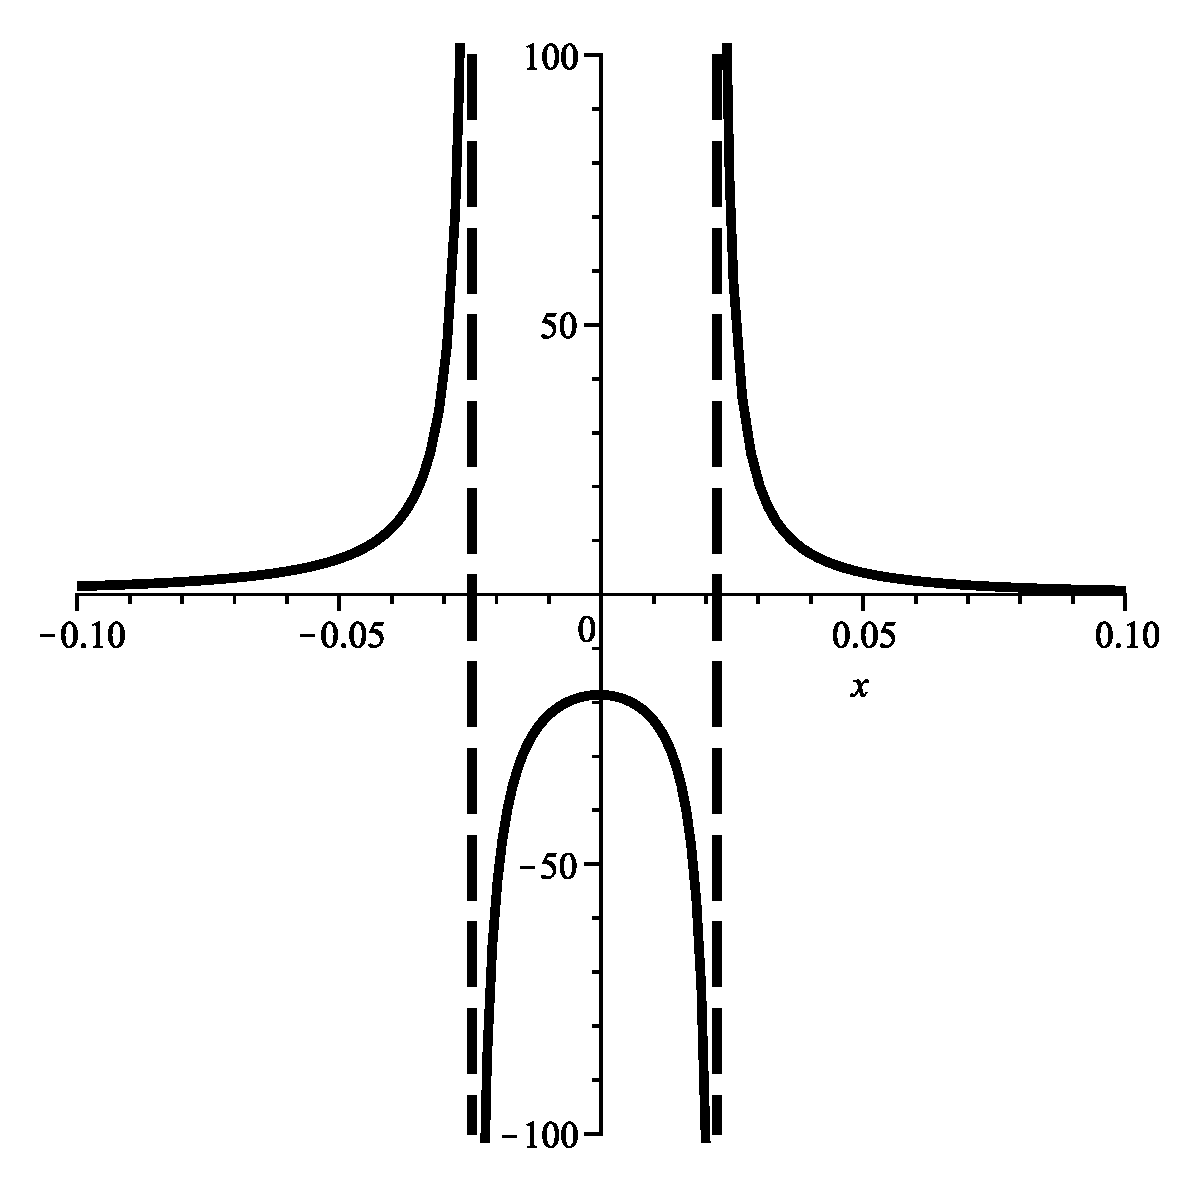
\includegraphics[scale=0.3]{figures/Picture.eps}}

% \caption{Another caption}
% \label{fig:Pict2}
% \end{figure}



% \subsection{Table}
% Lorem ipsum dolor sit amet, consetetur sadipscing elitr, sed diam nonumy eirmod tempor invidunt ut labore et dolore magna aliquyam erat, sed diam voluptua. At vero eos et accusam et justo duo dolores et ea rebum. Stet clita kasd gubergren, no sea takimata sanctus est Lorem ipsum dolor sit amet. Lorem ipsum dolor sit amet, consetetur sadipscing elitr, sed diam nonumy eirmod tempor invidunt ut labore et dolore magna aliquyam erat, sed diam voluptua. At vero eos et accusam et justo duo dolores et ea rebum. Stet clita kasd gubergren, no sea takimata sanctus est Lorem ipsum dolor sit amet\explainindetail{This needs further explanation}.
% \begin{table}[!ht]
% 	\centering
% 	\begin{tabular}{|l|rl|}
% 		\hline
% 		Something & Someother & Thing \\
%   		Seems & to be & good\\
%   		\hline
%   	\end{tabular}
%   	\caption{Random data for a table.}
% \end{table}

% Lorem ipsum dolor sit amet, consetetur sadipscing elitr, sed diam nonumy eirmod tempor invidunt ut labore et dolore magna aliquyam erat, sed diam voluptua. At vero eos et accusam et justo duo dolores et ea rebum. Stet clita kasd gubergren, no sea takimata sanctus est Lorem ipsum dolor sit amet. Lorem ipsum dolor sit amet, consetetur sadipscing elitr, sed diam nonumy eirmod tempor invidunt ut labore et dolore magna aliquyam erat, sed diam voluptua. At vero eos et accusam et justo duo dolores et ea rebum. Stet clita kasd gubergren, no sea takimata sanctus est Lorem ipsum dolor sit amet.


% \section{Model calibration}
% \subsection{What is calibration?}
% Here is an example of a matrix\citep{website:fermentas-lambda} in $A\in\mathcal{M}_n(\RR)$:
% $$
% A = 
% \begin{pmatrix}
% a_{11} & a_{12} & \ldots & a_{1n}\\
% a_{21} & \ddots & \ddots  & \vdots\\
% \vdots &  \ddots & \ddots  & \vdots\\
% a_{n1} &  \ldots &  \ldots & a_{1n}.
% \end{pmatrix}
% $$

% \subsection{Numerical methods for calibration}
...


